\documentclass{article}
\usepackage{graphicx} % Required for inserting images

% for setting up figures
\usepackage{subfigure}
\usepackage{multirow}

% package for margin spacing
\usepackage[margin=1.5in,inner=1.5in]{geometry}
\geometry{top=1.0in}

% package for math stuff
\usepackage{algorithmic}
\usepackage{algorithm}
\usepackage{mathtools}
\usepackage{amssymb}
\usepackage{amsmath}


\usepackage[style=authoryear]{biblatex}
\addbibresource{refs.bib}

\title{Meeting 31st March}
\author{Ben Hutchins}
\date{2023}

\begin{document}

\maketitle

\section*{Rossby waves}

\subsection*{Introduction}

Rossby waves are inertial waves which occur in rotating fluids due to the conservation of vorticity. In the atmosphere, these take the form of large-scale meanders in the high level winds which circle the poles. In the ocean they propogate along the thermocline and are caused by wind stress anomalies at the surface.

\subsection*{Physical basis}

Rossby waves occur in an inviscid, barotropic fluid of constant depth, such as the atmosphere.

\begin{itemize}
    \item Inviscid - viscous (frictional) forces are considered to be zero in the free atmosphere.
    \item Barotropic - surfaces of constant pressure and constant density coincide ($\nabla \rho \times \nabla p = 0$). Pressure depends only on density. 
\end{itemize}

In this case, the divergence of the horizontal velocity is zero, given by:

\begin{equation}
    \nabla_h \cdot \mathbf{\vec{u}} = \frac{\partial u}{\partial x} + \frac{\partial v}{\partial y} = 0
    \label{eq:divergence}
\end{equation}

The vorticity of the fluid is given by the curl of the velocity:

\begin{equation}
    \nabla \times \mathbf{\vec{u_a}} = \frac{\partial v}{\partial x} - \frac{\partial u}{\partial y} + f  = {\eta}
    \label{eq:absolute_vorticity}
\end{equation}

The absolute vorticity is given by the curl of the absolute velocity ($\mathbf{\vec{u_a}}$), which is the air velocity relative to an inertial frame. For this we consider only the vertical component of the relative vorticity, $\zeta = \frac{\partial v}{\partial x} - \frac{\partial u}{\partial y}$, and the vorticity of the earth, $f$ to give the absolute vorticity: $\eta = \zeta + f$.\\

For the barotropic, non-divergent (equation \ref{eq:divergence}) fluid case, the absolute vorticity is conserved following the motion:

\begin{equation}
    \frac{D}{Dt}(\zeta + f) = 0
    \label{eq:conservation_of_absolute_vorticity}
\end{equation}

% material derivative? having some issues with understanding this

In the more general case, we consider a baroclinic atmosphere where density depends on both temperature and pressure, where the geostrophic wind varies with height. In this case, the Rossby wave is a potential vorticity-conserving motion which occurs due to gradients in potential vorticity. The potential vorticity is given by:

\begin{equation}
    \mathcal{Q} = \alpha (2 \mathbf{\Omega} + \nabla \times \mathbf{u}) \cdot \nabla \theta
    \label{eq:potential_vorticity}
\end{equation}

Where $\mathbf{\Omega}$ is the angular velocity of the earth, $\alpha$ is the specific volume ($1/\rho$), $\mathbf{u}$ is the three dimensional vector velocity, and $\theta$ is the potential temperature ($\theta = T (p_0/p)^{\kappa}$). In the absence of friction and heating, the potential vorticity (ertel PV, $\mathcal{Q}$) is conserved following the motion of the fluid.\\

\subsubsection*{Emergence of Rossby waves \footnote[1]{Based on section 5.7 from \cite{holton_introduction_2013}}}

For an idealized case, we consider a barotropic fluid with a constant density and depth, where variation in the coriolis parameter is given by:

\begin{equation}
    f = f_0 + \beta y
    \label{eq:coriolis_parameter}
\end{equation}

Where:

\begin{description}
    \item[$f_0$] is the coriolis parameter at $\phi_0$, the latitude of the equator ($y=0$).
    \item[$\beta \equiv (df/dy)_{\phi_0} = 2 \Omega \cos{\phi_0/a}$]  is the Rossby parameter which accounts for the the meridional variation of the Coriolis force caused by the spherical shape of the earth. Where $\Omega$ is the angular velocity of the earth, and $a$ is the radius of the earth.
    \item[$y$] is the distance from the equator.
\end{description}

This equation describes how the coriolis paramater varies linearly with latitude and is known as the beta-plane approximation.\\

To understand the emergence of Rossby waves we can consider a chain of air parcels encircling a band of latitude. If we consider the absolute vorticity given by $\eta = \zeta + f$, where $\zeta$ is the relative vorticity ($\zeta = \partial v / \partial x - \partial u / \partial y$) and f is the Coriolis parameter. Initially, when t=0, $\zeta = 0$. At time t=1, a meridional displacement is applied to to the air parcels, $\delta y$, whereby the parcels are displaced from their original latitude. At time t=1:

\begin{equation}
    (\zeta + f)_{t=1} = f_{t=0}
    \label{eq:zeta}
\end{equation}

Using equation \ref{eq:coriolis_parameter}, we can write:

\begin{equation}
    \zeta_{t=1} = f_{t=0} - f_{t=1} = f_{t=0} - (f_{t=0} + \beta \delta y) = -\beta \delta y
    \label{eq:zeta_rearanged}
\end{equation}

Where $\beta \equiv \partial f/ \partial y$ gives the planetary vorticity gradient.\\

% why would this meridional displacement be sinusoidal?

If this chain of air parcels is subjected to a sinusoidal meridional displacement, with absolute vorticity connservation, the resulting perturbation to the absolute vorticity will be positive for a southern displacement ($\delta y < 0$) and negative for a northern displacement ($\delta y > 0$).\\

% restoration gradient

This perturbation to the vorticity will lead to a change in the meridional velocity field, which will advect the chain of parcels southward to the west of the vorticity maxima and northward to the west of the vorticity minimum. This causes the air parcels to oscillate back and forth about the latitude band while the vorticity maxima and minima propogate to the west. This westward-propogating vorticity field is the Rossby wave. In a similar way to how vertical gradients of potential temperature resist vertical fluid displacements, the meridional gradient of absolute vorticity resists meridional fluid displacements and provides a restoring mechanism for Rossby waves.\\

The speed of propogation, $c$, can be computed in the example by setting $\delta y = a \sin[k(x - ct)]$ and taking the total derivative $v = D(\delta y)/Dt = -kca \cos[k(x - ct)]$. Considering the x component of the relative vorticity in equation \ref{eq:zeta}, we can write:

\begin{equation}
    \zeta  = \frac{\partial v}{\partial x} = k^2 ca \cos[k(x - ct)]
    \label{eq:zeta_x}
\end{equation}

By substituting $\delta y$ and $\zeta$ into equation \ref*{eq:zeta_rearanged} we can write:

\begin{equation}
    k^2 ca \cos[k(x - ct)] = -\beta a \sin[k(x - ct)]
    \label{eq:zeta_x_substitution}
\end{equation}

Solving for $c$ we get:

\begin{equation}
    c = -\frac{\beta}{k^2}
    \label{eq:zeta_x_substitution_c}
\end{equation}

Therefore, the phase speed, $c$, is westward relative to the mean flow and is inversely proportional to the square of the zonal wavenumber, $k$.\\
 
The group velocity ($\frac{\partial \omega} {\partial k}$) for the special case of the one-dimensional wave ($l=0$) is given by\footnote[2]{From Danny Feltham's fluid dynamics notes}:

\begin{equation}
    c^{(x)}_{group} = U + \frac{\beta}{k^2}
    \label{eq:group_velocity}
\end{equation}

Where $U$ is the mean zonal velocity. The group velocity in equation \ref{eq:group_velocity} is therefore eastward relative to the mean flow for the $k>l$ case.\\

% why is this important? 

%\subsection*{Free Barotropic Rossby Waves}

% more formal definition by finding wave-type solutions of the linearized barotropic vorticity equation

% see section 5.7.1 of Holton for this
% or the wikipedia page
% or in the Vallis fluid dynamics book


\subsection*{Relevance}

Rossby waves in the atmosphere are typically observed as (between 4-6) large scale meanders in the jet stream. When these meanders become detached, they form cylones (+ve vorticity) and anticylones (-ve vorticity). Rossby wave breaking can be diagnosed from the formation of elongated potential vorticity (PV) filaments, which are referred to as PV streamers, which can eventually split into cutoffs and lead to the formation of blocking highs over Europe \cite{deVries2021}. These events are significant for the power-sector in Europe as they can lead to sustained periods of cold and still conditions, which cause a reduction in wind power generation along with increased demand.\\

 

\section*{Eddy mean flow}

Synoptic eddies are small scale disturbances in the atmosphere which are generated by baroclinic instability, driven by meridional temperature gradients. These can propogate away from the zones of baroclinic instability in which they are generated and converge with momentum in the midlatitudes. This can act to produce and maintain the midlatitude westerly jet, which is also known as the eddy-driven jet \cite{sang_evaluation_2022}. \\

By considering how baroclinic eddies can generate Rossby waves by mid-latitude stirring, we can understand how eddy momentum flux maintains the mean flow.\\

\subsection*{Rossby waves and momentum convergence\footnote[3]{Based on section 2.4.4. from ACP's Global Circulation notes.}}

As Rossby waves form due to gradients of PV, the disturbances generated by baroclinic instability will generate Rossby waves in the mid-latitudes. Once the flow is disturbed, these waves will propogate away from the source region. If we assume that the waves are approximately linear and don't interact with one another, we can represent the waves using the horizontal streamfunction.

\begin{equation}
    \psi = \text{Re} \biggl( A e^{i(kx + ly - \omega t)}\biggr)
    \label{eq:streamfunction}
\end{equation}

We consider the zonal and meridional velocities as the y and x derivatives of the streamfunction, respectively:

\begin{align*}
    u = - \frac{\partial \psi}{\partial y} \\
    v = \frac{\partial \psi}{\partial x}
    \label{eq:uv_streamfunction}
\end{align*}

As the velocity components have no zonal mean component, as they represent an oscillating wave around the mean flow, we consider the eddy ($u^*$ and $v^*$) terms only:

\begin{align*}
    u^* = -\text{Re} \biggl( A il e^{i(kx + ly - \omega t)}\biggr) \\
    v^* = \text{Re} \biggl( A ik e^{i(kx + ly - \omega t)}\biggr)
    \label{eq:uv_eddy}
\end{align*}

To get the momentum flux we need to multiply these terms together and take the zonal mean. We can do this by using Euler's formula to write the complex exponential as a sum of two trigonometric functions: $e^{i\theta} = \cos(\theta) + i \sin(\theta)$ and define $\theta = kx + ly - \omega t$. Considering the zonal component first:

\begin{align*}
    u^* &= -\text{Re} \biggl( A il (\cos(\theta) + i \sin(\theta))\biggr) \\
    u^* &= -\text{Re} \biggl( Al(i\cos{\theta} - \sin{\theta})\biggr) \\
    u^* &= A l \sin{\theta}
    \label{eq:u_eddy}
\end{align*}

Then for the meridional mean:

\begin{equation}
    v^* =-Ak \sin{\theta}v*
    \label{eq:v_eddy}
\end{equation}

Then multiplying these together and taking the zonal mean:

\begin{align*}
    u^* v^* &= -A^2 l k \sin^2{kx + ly - \omega t} \\
    u^* v^* &= -A^2 l k \biggl( \frac{1}{2} - \frac{1}{2} \cos{2(kx + ly - \omega t)} \biggr) \\
    [u^* v^*] &= -A^2 l k \biggl( \frac{1}{2 \pi} \int_{0}^{2 \pi} \frac{1}{2} - \frac{1}{2} \cos{2(kx + ly - \omega t)} \biggr) \\
    [u^* v^*] &= -A^2 l k \bigl( \frac{\pi}{2 \pi} \bigr) \\
    [u^* v^*] &= -\frac{1}{2} A^2 l k
    \label{eq:uv_eddy_zonal_mean}
\end{align}

Therefore the momentum flux due to the Rossby waves depends on the $kl$ terms, the zonal and meridional wavenumbers. From this an expression can be described for the meridional group velocity of the Rossby waves:

\begin{equation}
    c^{(y)}_{group} = \frac{2 \beta k l }{(k^2 + l^2)^2}
    \label{eq:group_velocity}
\end{equation}

The Rossby waves considered transport energy away from the baroclinic source region in the meridional direction given by the group velocity, the direction of which is determined by the sign of the $kl$ terms. If the $kl$ terms are positive, northward of the source region, the momentum flux given by $[u^* v^*]$ will be negative, and so the direction of the flux will be southward . If the $kl$ terms are negative, southward of the source region, the momentum flux given by $[u^* v^*]$ will be positive, and so the direction of the flux will be northward. As a result, the momentum flux associated with Rossby waves converges towards the source region. \\

The opposite is true for the group velocity, given in equation \ref{eq:group_velocity}. If the $kl$ terms are positive, northward of the source region, the group velocity will be positive, so Rossby waves will break and dissapate northward of the source region. If the $kl$ terms are negative, southward of the source region, the group velocity will be negative, so Rossby waves will break and dissapate southward of the source region. The Rossby waves therefore transport energy away from the disturbance (source region). This is visualised in figure \ref{fig:rossby_waves}.

\begin{figure}[h]
    \centering
    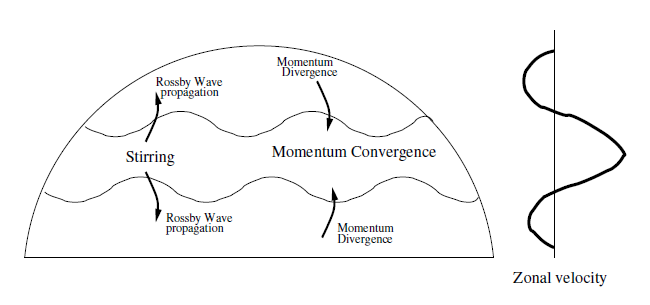
\includegraphics[width=0.5\textwidth]{eddy-driven-jet.png}
    \caption{Schematic from ACP's Global Circulation notes showing the momentum flux associated with Rossby waves propogating away from a region of stirring.}
    \label{fig:rossby_waves}
\end{figure}

\subsection*{Relevance}

Eddies driven by baroclinic instability are important for decadal forecasting and energy systems as they drive the weather. Eddy influences on the midlatitude jet can be significant for large-scale conditions over Europe, depending on how the eddies act to amplify or dampen the jet.

% waffle waffle waffle

\section*{PhD update}

% short term goals
% longer term goals
% deliverables - presentations/MC2
% research ideas and questions



% what is the mechanism for this in the oceans
% gain momentum from wind stress at the ocean surface

\printbibliography

\end{document}
